\white{May 2024}
\begin{center}
    \begin{tikzpicture}
        % Define the dimensions of the calendar
        \def\year{2024}
        \def\month{5}
        \def\monthname{May}
        \def\startday{3} % 1=Sunday, 2=Monday, ..., 7=Saturday
        \def\numdays{31}
        \def\boxwidth{2} % Width of each box
        \def\boxheight{1.8} % Height of each box

\newcommand{\daytext}[1]{
    \ifcase#1
    \or Practice \or \cross \or Practice \or  \cross \or  \cross \or  \cross \or  \cross \or Practice \or  \cross \or Practice
    \or  \cross \or  \cross \or  \cross \or  \cross \or Practice \or  \cross \or Practice \or  \cross \or  \cross \or \cross
    \or  \cross \or Practice \or  \cross \or Practice \or  \cross \or  \cross \or  \cross \or  \cross \or Practice \or  \cross
    \or Practice
    \fi
}

        % Draw the calendar grid
        \foreach \x in {0, 1, 2, 3, 4, 5, 6, 7} {
            \draw (\x*\boxwidth, 0) -- (\x*\boxwidth, -6*\boxheight);
        }
        \foreach \y in {0, -1, -2, -3, -4, -5, -6} {
            \draw (0, \y*\boxheight) -- (7*\boxwidth, \y*\boxheight);
        }

        % Add day labels
        \node at (0.5*\boxwidth, 0.5*\boxheight) {Sunday};
        \node at (1.5*\boxwidth, 0.5*\boxheight) {Monday};
        \node at (2.5*\boxwidth, 0.5*\boxheight) {Tuesday};
        \node at (3.5*\boxwidth, 0.5*\boxheight) {Wednesday};
        \node at (4.5*\boxwidth, 0.5*\boxheight) {Thursday};
        \node at (5.5*\boxwidth, 0.5*\boxheight) {Friday};
        \node at (6.5*\boxwidth, 0.5*\boxheight) {Saturday};

        % Add the dates in the top left corner and specific text in the middle
        \foreach \d in {1,...,\numdays} {
            \pgfmathtruncatemacro{\col}{mod(\d+\startday-2, 7)}
            \pgfmathtruncatemacro{\row}{-(\d+\startday-2)/7}
            \node[anchor=north west] at (\col*\boxwidth, \row*\boxheight) {\d};
            \node[anchor=center, text width=\boxwidth cm, align=center] at (\col*\boxwidth+0.5*\boxwidth, \row*\boxheight-0.5*\boxheight) {\daytext{\d}};
        }

        % Add month and year
        \node at (3.5*\boxwidth, 1.5*\boxheight) {\textbf{\monthname\ \year}};
    \end{tikzpicture}
\end{center}

This is our what happened during the month of May. We had full team meetups every Tuesday and every Thursday. Connor had the robot during this time. At the end of the month we had just started building the Drivetrain.
\white{Team Biographies (May 2, 2024)}
\label{Team-Biographies}
\chapterauthor{Caleb Bachmeier}
\info{Caleb Bachmeier}{Team Biographies}{May 2, 2024}
\label{team-bios}
\textbf{Goal}: Breakdown the team's members

    \section*{7686X: Phoenix Rising}
    We are a VRC team out of Harrisburg, South Dakota. This year is our second second year competing as a team, in the 2023-2024 season we won the Innovate Award at South Dakota State Championship, while also making some excellent coding research which will be talked about later in this notebook.
   \section*{Connor Albers }
I am Connor Albers , this will be seventh year competing in VEX robotics, and I am in 10th grade at Harrisburg High School in Harrisburg South Dakota. I am the lead engineer of the robot.
\label{connor}
   \section*{Caleb Bachmeier}
I am Caleb Bachmeier, this will be my seventh year competing in VEX robotics,  and I am in 10th grade at Harrisburg High School in Harrisburg South Dakota. I am the team captain and document everything the team is doing in this engineering notebook. 
\label{Caleb}
   \section*{Miles Berger}
I am Miles Berger, this will be my seventh year competing in VEX robotics, and I am in 10th grade at Harrisburg High School in Harrisburg South Dakota. I am the backup driver for the team. 
\label{Miles}
   \section*{Chase Blake}
I am Chase Blake, this will be my fourth year competing in VEX robotics, and I am in 10th grade at Harrisburg High School in Harrisburg South Dakota. I am the main driver for the team but, when I am not driving, I research what other teams are doing to solve this year's challenge. 
\label{Chase}
   \section*{Ian Smith}
I am Ian Smith, this will be my second year competing in VEX robotics, and I am in 10th grade at Harrisburg High School in Harrisburg South Dakota. I am 1 of the 2 coders our team has and I mainly focus on integrating Jayden's code into the main drive program as well as finding the best ways for our driver to effectively control the robot. 
\label{Ian}
   \section*{Jayden}
I am Jayden, this will be my seventh year competing in VEX robotics, and I am in 10th grade at Harrisburg High School in Harrisburg South Dakota. I am 1 of the 2 coders our team has and I mainly focus on innovative ways our team can automate our robot. 
\label{Jayden}
\begin{center}
    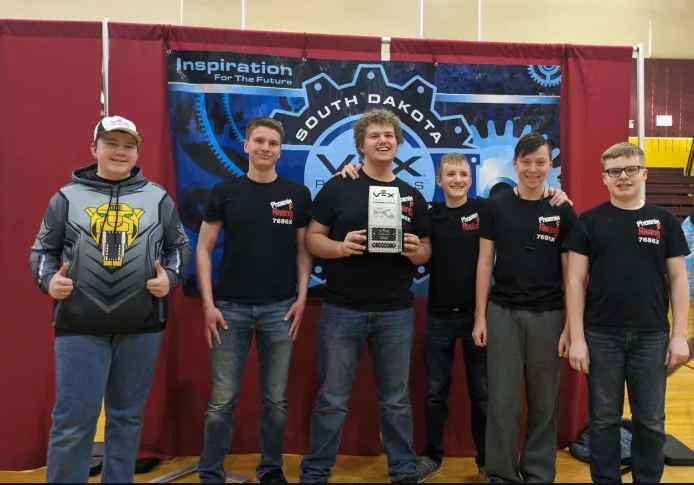
\includegraphics[width=0.9\linewidth]{images/Innovate wo Ezra.png}
    \captionof{figure}{Innovate at SD State} % Use \captionof instead of \caption
    \label{fig:innovate}
\end{center}

\white{Team Goals (May 5, 2024)}
\label{Team-Goals}
\chapterauthor{Caleb Bachmeier}
\info{Caleb Bachmeier}{Team Goals}{May 5, 2024}
{
\textbf{Goal}: Explain the team's goals for the High Stakes season
\section*{Team Goals}
\begin{itemize}
    \item \textbf{Learn something new}
    
    This might be our most important goal all season. Learning more is the only way to get better. We learned a lot last season through coding, building, driving, and notebooking. Even if it means we fail, learning not to make the same mistake twice is the best thing we can do.
    
    \item \textbf{Win a banner at a signature event}
    
    This would be an astounding achievement as banners at signature events are very hard to obtain. This would also make us much more appealing to future alliance partners, and they also look really neat.
    
    \item \textbf{Qualify for the World Robotics Competition }
    
    Qualifying for Worlds would be exceptional for the team. This has been a lifelong dream for us because it would allow us to show more teams what we can do. 
    
    \item \textbf{Win 85\% or more of qualification matches}
    
    This would place us higher in rankings. While it is an ambitious goal, the team thinks that it is one we should strive for, in order to get our name out there and hopefully gain better alliances in the future. 
    
    \item \textbf{Utilize all scoring methods of the game}
    
    When designing our robot, it is imperative to consider all approaches of the game. This will also help us better align ourselves with an alliance partner that compliments us best.

    \item \textbf{Be safe}

    Our safety goal is to operate our robot with precision and care. We commit to wearing safety glasses, respecting field boundaries, and avoiding unsafe actions. By prioritizing safety, we contribute to a positive and secure environment for all teams in the VEX VRC.
\end{itemize}
}
\white{Identify Game Problem (May 8, 2024)}
\label{Identify-Game-Problem}
\chapterauthor{Caleb Bachmeier}
\info{Caleb Bachmeier}{Identify Game Problem}{May 8, 2024}
\textbf{Goal}: Breakdown the High Stakes Game Manual Version 1.0
\section*{Field Analysis}
{
\textbf{Goal:} Analyze VEX VRC's game "High Stakes" (Figure \blueref{fig:high-stakes-field}{High Stakes Field})
\begin{itemize}
\item There are forty-eight rings on the field (Figure \blueref{fig:red-ring}{Ring Red})
\item Rings have an outer diameter of seven inches, inner diameter of three inches, and a thickness of two inches 
\item There are five hexagonal mobile goals on the field (Figure \blueref{fig:red-ring}{Ring Red}) 
\item Hexagonal mobile goals are ten inches wide and fourteen and a half inches tall
\item There are ten stakes you can score on, five hexagonal mobile goals, two alliance stakes, two wall stakes, and one stake on the four foot tall ladder 
\item On all stakes every ring is worth 1 point, except for the highest ring on the stake, which is worth three points
\item During the fifteen second autonomous period, you must stay on your alliances side.
\item Autonomous Win Point (AWP) is very useful for climbing up rankings as we have discovered in previous years
\item \hl{AWP at least three rings scored, two stakes with at least one ring scored.}
\item One robot can only carry two rings and one stake at a time. Rings scored on a goal that is being carried does not count against the two ring limit.
\item Rings can be descored at any time 
\item There is a four foot ladder in the middle of the field with three rings on it 
\item There are three levels on the ladder. Getting off of the ground gets you three points, passing above the first bar gets you six points, passing the second par gets you twelve points 
\item Robots can climb on any side of the ladder 
\item Between the four corners on the field, two are "positive corners" and the other two are "negative corners" teams can move mobile goals into these corners to change the scores on the mobile goals 
\item A positive corners multiplies the stakes points. For example, if I had a stake with six red rings on it, normally that stake would be worth 8 points, but if I put it into a positive corner, that stake would be worth 16 points, for the time that the stake is in the corner
\item A negative corner effectively makes the point values negative. For example, if I had a stake with six blue rings it would be worth an additional eight points for the blue alliance, but if I put that mobile goal into a negative corner, all points are negative and the mobile goal would be worth negative eight points for the blue alliance (Note: you can not have negative points at the end of the match, zero points is the lowest you can have)
\end{itemize}
\begin{figure}[hbt!] % Use [hbt!] to place the figures on the same page
    \begin{minipage}{.5\textwidth}
        \centering
        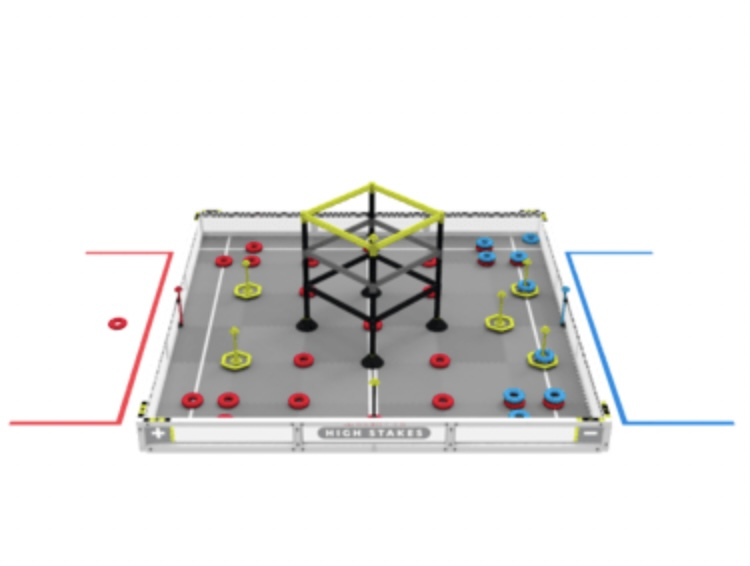
\includegraphics[width=.8\linewidth]{images/High Stakes Field.jpeg}
        \caption{High Stakes Field}
        \label{fig:high-stakes-field}
    \end{minipage}
    \begin{minipage}{.5\textwidth}
        \centering
        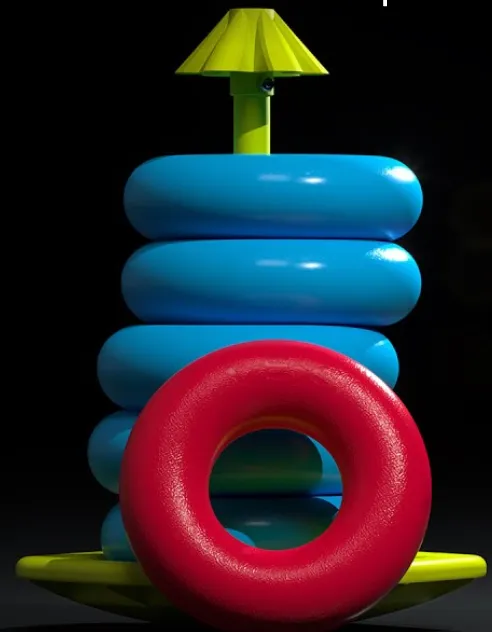
\includegraphics[width=.8\linewidth]{images/Stake.png}
        \caption{Mobile Goal with Rings}
        \label{fig:stake}
    \end{minipage}
    \begin{minipage}{.5\textwidth}
        \centering
        
\includegraphics[width=.8\linewidth]{images/Red Ring.jpeg}
        \caption{Red Ring}
        \label{fig:red-ring}
    \end{minipage}
\end{figure}
}
\section*{Important Terms}
    \subsection*{Game Objects}
    \begin{itemize}
    \item Rings (Figure \blueref{fig:red-ring}{Ring Red})
    \item Mobile Goals (Figure \blueref{fig:stake}{Stake})
    \end{itemize}
    \subsection*{Match Play}
    \begin{itemize}
        \item \textbf{Starting Line}: The location where robots are placed at the beginning of a match.
        \item \textbf{Autonomous Period}: A segment of the match where robots operate and score points using pre-programmed instructions without any driver input. This section of the match takes place in the first fifteen seconds of the match.
        \item \textbf{Driver Control}: This is the phase following the autonomous period where drivers control their robots to score points. This section of the match is ninety-five seconds long.
        \item \textbf{Endgame}: The final fifteen seconds of the match where teams can score additional points, often through specific tasks. This year by climbing a four foot tall ladder.
    \end{itemize}
    \subsection*{Violations}
    \begin{itemize}
\item \textbf{Minor Violation} - A Violation which does not result in a Disqualification

\item \textbf{Major Violation} - A Violation which results in a Disqualification

\item \textbf{Match Affecting} - A Violation which changes the winning and losing AllIance in the Match 

\item \textbf{Entanglement} - A Robot is Entangled if it has grabbed, hooked, or attached to an opposing Robot or a Field Element.

\item \textbf{Holding} - A Robot status, a robot is considered to be Holding if it meets any of the following criteria during match:
\begin{itemize}
    \item Trapping: Limiting the movement of an opponent Robot to a small or confined area of the field, approximately the size of one foam field tile or less, without any avenue for escape. \hl{(If a robot is not attempting to escape it is NOT trapped.)}
    \item Pinning: Preventing the movement of an opponent Robot through contact with the Field Perimeter, a Field or Game Element, or another Robot.
    \item Lifting: Controlling an opponent's movements by raising or tilting the opponents robot off of the foam tiles 
\end{itemize}
    \end{itemize}
\section*{Understanding Game Rules \vexManual}
%<SG> Rules 
{
\begin{itemize}
\item
\textbf{\textless SG1\textgreater} Starting a Match

- Prior to the start of each Match, the robot must be placed so that it is:
\begin{itemize}
    \item Contacting / breaking the plane of their Alliance's Starting Line
    \item Not contacting any scoring objects, with any exception of one Preload that is touching the robot
    \item Not contacting any other Robots 
    \item Completely stationary (i.e., no motors or any other mechanisms in motion)
\end{itemize}

- If an robot does not meet these requirements within a reasonable amount of time the robot is Disqualified from the match 
\item
\textbf{\textless SG2\textgreater} Horizontal expansion is limited

- Once the Match begins, Robots may expand outside of the 18" x 18" starting size, but the may never expand outside of the 24" x 18" size 

- From the robots perspective, it may only expand from one direction (from a single side of the robot)
\item
\textbf{\textless SG3\textgreater} Vertical expansion is limited

- Once the Match begins robots may expand vertically, but may never be breaking the plane of more than two Levels of the Ladder at any given time. \texthl{(This basically is a height limit of 32")} 
Game
- The floor is considered a Level 
\item
\textbf{\textless SG4\textgreater} Keep Scoring Objects in the field 

- Teams may not intentionally nor strategically remove Scoring Objects

- Any Rings that leave the Field during the Match will be given to the same Drive Team Members from the same color Alliance as the rings.
\item
\textbf{\textless SG5\textgreater} Each Robot gets one Ring as a preload 

- Prior to the start of the Match each preload must be contacting a robot of the same color as the preload 
\item
\textbf{\textless SG6\textgreater} Possession is limited to two Rings and one Mobile Goal

- If your robot has over this limit, it must stop all actions other than that of getting rid of the excess objects

- Rings on a mobile goal that you are carrying does not count against the ring count \texthl{(I.e. if your robot is carrying a mobile goal with six rings scored on it and is carrying two rings separately that would be legal.)}
\item
\textbf{\textless SG7\textgreater} Don't cross the Autonomous Line

- During the Autonomous period, Robots can not touch the foam tiles, Scoring Objects, or Field Elements which are on the opposing Alliance's side of the Autonomous Line \texthl{(Wall Stakes or Scoring Objects are on neither side of the line, both teams can come in contact with them)}

\item
\textbf{\textless SG8\textgreater} Engage with the Autonomous Line at your own risk 

- Any Robot who engages with Scoring Objects and/or the Wall Stakes on the Autonomous line should be aware that opponent Robots can do the same. 
\item
\textbf{\textless SG9\textgreater} Don't remove opponents from the ladder 

- There isn't a rule that explicitly states that incidental contact is prohibited; however, you can not intentionally pull a robot down from climbing 
\item
\textbf{\textless SG10\textgreater} Alliance Wall Stakes are protected

- Alliances can not directly nor indirectly interact with an opponent's Alliance Wall Stake. This includes Scoring and Descoring 
\item 
\subsection*{Update to Judging: June 26th}
\textbf{\textless SG11\textgreater} Positive corners are "safe" during the endgame

- During the last ten seconds of a Match, Robots may not contact Mobile Goals in the Positive Corners of the Field, and may not add or remove Mobile Goals or Rings to or from the Positive Corners of the field
\end{itemize}
}
\white{Game Strategies (May 10, 2024)}
\label{Game-Strategies}
\chapterauthor{Chase Blake}
\info{Chase Blake}{Game Strategies}{May 10, 2024}
\textbf{Goal}: Identify offensive and defensive game strategies
    \section*{Game Strategy}
    \textbf{Goal}:
    We will develop game strategies for this year's game so that we can have a better understanding of what we may encounter in game

    \textbf{Scoring Prioritization}:
    Admittedly, this is going to be a very odd year for scoring because of the positive and negative corners. We will count negative points against our opponents as positive points for us.

    \textbf{Scoring Method Points}:
    \begin{itemize}
        \item Eight points for a fully stacked stake
        \item Sixteen points for a fully stacked stake in any of the corners 
        \item Three points for getting off of the ground using the ladder 
        \item Six points for passing the first rung of the ladder
        \item Twelve points for passing the second rung of the ladder 
    \end{itemize}
    \centering \textbf{On the following page there is a bar graph of point breakdown}
    \pagebreak
    \begin{figure}[t!]
        \centering
        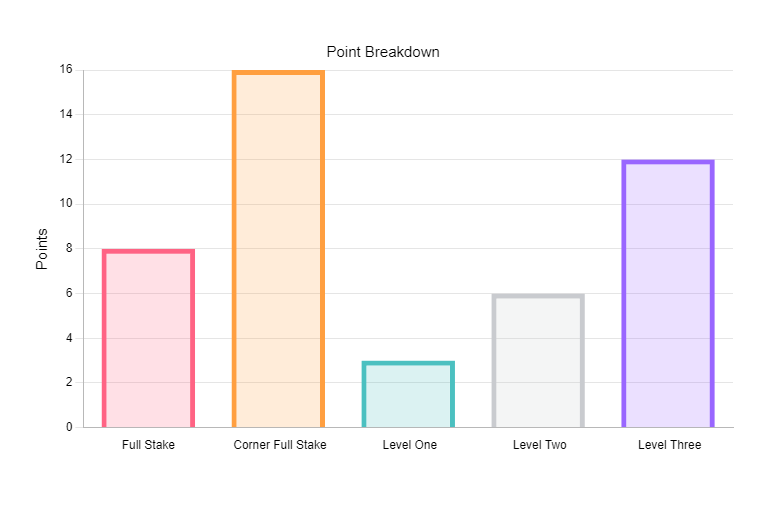
\includegraphics[width=1\textwidth]{images/Point Breakdown .jpg}
        \caption{Point Breakdown}
        \label{fig:point-breakdown}
    \end{figure}
    
    \section*{Offensive Strategies}
\noindent
    \textbf{Defending a full stake in the negative corner}:

\noindent
\textbf{Pros}:
\begin{itemize}
    \item Guaranteed negative eight points for the opposing alliance 
\end{itemize}
\textbf{Cons}:
\begin{itemize}
    \item Loses out on all other opportunities to score points 
\end{itemize}

    \textbf{Descoring opponent's stakes}:

\noindent
\textbf{Pros}:
\begin{itemize}
    \item Makes the opponents attempts to score futile 
\end{itemize}
\textbf{Cons}:
\begin{itemize}
    \item Loses out on other opportunities to score points 
\end{itemize}
    \section*{Defensive Strategies}
    \noindent
    \textbf{Hanging as soon as possible}:

\noindent
\textbf{Pros}:
\begin{itemize}
    \item Guaranteed Twelve Points for a Level 3 hang
\end{itemize}
\textbf{Cons}:
\begin{itemize}
    \item Loses out on other opportunities to score additional points 
\end{itemize}

\noindent
    \textbf{Defending a full stake in the additional corner}:

\noindent
\textbf{Pros}:
\begin{itemize}
    \item Guaranteed Sixteen Points 
\end{itemize}
\textbf{Cons}:
\begin{itemize}
    \item Loses out all opportunities to score additional points 
\end{itemize}

\noindent
    \textbf{Defending a stake, then hanging at the end of the match}:

\noindent
\textbf{Pros}:
\begin{itemize}
    \item If us and our allIance partner does this a point maximum is 56 points
\end{itemize}
\textbf{Cons}:
\begin{itemize}
    \item High risk, high reward. If when we leave to go hang one of our opponents goes to descore our stakes the bulk of our points would be lost  
\end{itemize}
\white{Gantt Chart (May 13, 2024)}
\label{Gantt-Chart}
\chapterauthor{Caleb Bachmeier}
\info{Caleb Bachmeier}{Gantt Chart}{May 13, 2024}
\textbf{Goal}: Identify our timeline for the High Stakes season
\section*{Gantt Chart: May 2024 - October 2024}

    The Gantt Chart below (\blueref{may-gantt-chart}{May Gantt Chart}) covers the time frame from May of 2024 (the beginning of our season) to October of 2024. These are our goals for the season. Our biggest goal is finishing our first robot by the end of July, this will allow for about  three months of drive time for our drivers, \blueref{Chase}{Chase} and \blueref{Miles}{Miles}, before our first tournament which will be in October
\begin{figure}[H]
    \begin{center}
        \begin{ganttchart}[
            y unit title=0.4cm,
            y unit chart=0.5cm,
            vgrid,
            hgrid,
            title label anchor/.style={below=-1.6ex},
            title left shift=.05,
            title right shift=-.05,
            title height=1,
            progress label text={},
            bar height=0.7,
            group right shift=0,
            group top shift=.6,
            group height=.3
        ]{1}{24} % Number of weeks
            % Labels
            \gantttitle{Week}{24} \\
            \gantttitle{May}{4}
            \gantttitle{June}{4}
            \gantttitle{July}{4}
            \gantttitle{August}{4}
            \gantttitle{September}{4}
            \gantttitle{October}{4}\\
            % Tasks
            \ganttbar{Set Up}{1}{2} \\
            \ganttbar{Build 1st Robot}{3}{12} \\
            \ganttbar{Program 1st Robot}{8}{12} \\
            \ganttbar{Improve 1st Robot}{13}{24} \\
            \ganttbar{Drive 1st Robot}{13}{24} \\
            % Relations \ganttlink{elemx}{elemy}

        \end{ganttchart}
    \end{center}
    \caption{Gantt Chart}
    \label{may-gantt-chart}
\end{figure}
\pagebreak
\section*{Gantt Chart: November 2024 - April 2025}

    The Gantt Chart below (\blueref{november-gantt-chart}{November Gantt Chart}) covers the time frame from November of 2024 to April of 2025 (the end of our season). Our main goal is to finish building our second robot by New Years. This will ensure that our robot will be ready to be driven to prepare for the rest of our qualification tournaments. Our third robot will be our state tournament, U.S. Open, and our Worlds robot. 
    \begin{figure}[H]
    \begin{center}
        \begin{ganttchart}[
            y unit title=0.4cm,
            y unit chart=0.5cm,
            vgrid,
            hgrid,
            title label anchor/.style={below=-1.6ex},
            title left shift=.05,
            title right shift=-.05,
            title height=1,
            progress label text={},
            bar height=0.7,
            group right shift=0,
            group top shift=.6,
            group height=.3
        ]{1}{24} % Number of weeks
            % Labels
            \gantttitle{Week}{24} \\
            \gantttitle{November}{4}
            \gantttitle{December}{4}
            \gantttitle{January}{4}
            \gantttitle{February}{4}
            \gantttitle{March}{4}
            \gantttitle{April}{4}\\
            % Tasks
            \ganttbar{Improve 1st Robot}{1}{8} \\
            \ganttbar{Drive 1st Robot}{1}{8} \\
            \ganttbar{Build 2nd Robot}{1}{8} \\
            \ganttbar{Program 2nd Robot}{4}{10} \\
            \ganttbar{Improve 2nd Robot}{8}{13} \\
            \ganttbar{Drive 2nd Robot}{8}{13} \\
            \ganttbar{Build Final Robot}{10}{16} \\
            \ganttbar{Improve Final Robot}{16}{24} \\
            \ganttbar{Drive Final Robot}{16}{24} \\
        \end{ganttchart}
    \end{center}
    \caption{Gantt Chart}
    \label{november-gantt-chart}
    \end{figure}
\white{Skills Rules (May 14, 2024)}
\label{skills-rules}
\chapterauthor{Miles Berger}
\info{Miles Berger}{Skills Rules}{May 14, 2024}
\section*{Overview of VEX Skills}
The VEX Robotics Competition (VRC) includes a variety of challenges designed to test the skills and creativity of participants. One of the key components is the Robot Skills Challenge, which consists of two parts: Driver Skills and Programming Skills. In Driver Skills, the robot is controlled by a driver to score as many points as possible within a set time. In Programming Skills, the robot operates autonomously using pre-written code to achieve the highest score possible. These challenges encourage students to develop their programming and driving skills, as well as their strategic thinking and problem-solving abilities.

\section*{High Stakes Season Skills Rules}
The High Stakes season introduces several unique changes to the Skills Challenge rules compared to previous seasons. One of the most notable differences is the new field layout, where Positive Corners and Negative Corners are now on the same side of the field, rather than being cater-cornered. This change affects the strategy for both Driver Skills and Programming Skills, as teams must now navigate the field differently to maximize their scoring potential. Additionally, the High Stakes season includes a new rule that adds a 2-point bonus per Climb for whichever alliance has Rings scored on the High Stake at the end of a match. This incentivizes teams to focus on scoring Rings on the High Stake, adding a new layer of complexity to the Skills Challenge.

Another significant change is the clarification and expansion of several existing rules. For example, the definition of "Plowing" has been rewritten, and new figures have been added to clarify the intent of specific rules. The rules for preloads have also been updated to ensure that they cannot start in a scored location or in contact with Stakes. These changes aim to provide clearer guidelines and prevent any ambiguities that could affect the outcome of matches. Overall, the High Stakes season's Skills Challenge rules emphasize strategic planning and precise execution, making it a more challenging and engaging competition for teams.

\section*{Scoring Rules for Red and Blue Rings}
In the High Stakes season, the scoring rules for red and blue rings have been updated to add more strategic depth to the game. Each ring scored on a stake is worth one point, while the top ring on each stake is worth three points. Additionally, mobile goals can be placed into Positive Corners or Negative Corners to change the values of the rings on that goal. This means that teams must carefully plan their ring placements to maximize their scores.


Furthermore, the rules specify that for a blue ring to have a point value in any position, all 24 red rings must be scored on stakes and have point values at the end of the match. This adds an extra layer of complexity, as teams must ensure that all red rings are properly scored before blue rings can contribute to their total score. These changes encourage teams to develop more sophisticated strategies and enhance the overall challenge of the Skills Competition.

\begin{figure}[!ht]
    \centering
    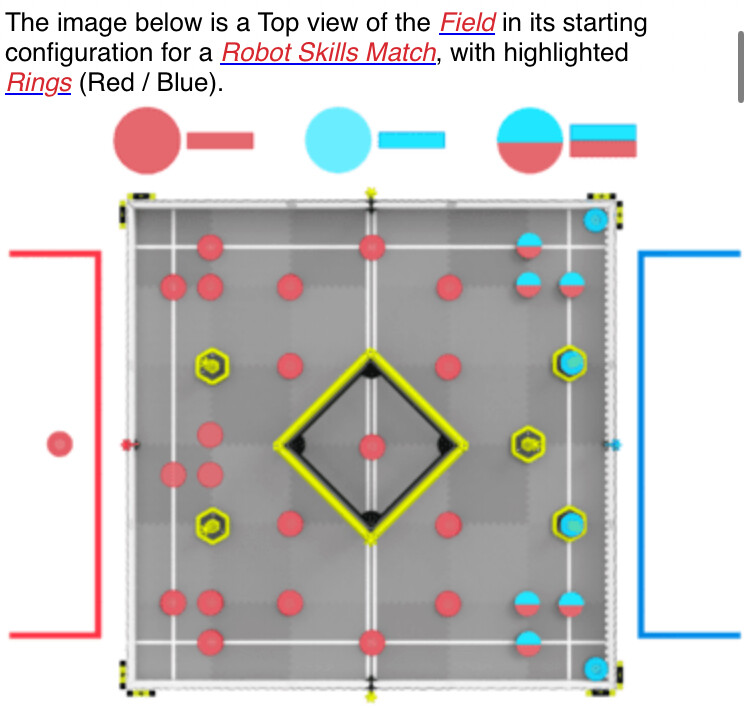
\includegraphics[width=0.5\linewidth]{images/SkillsFieldHighStakes.jpeg}
    \caption{Skills Field}
    \label{fig:skillsfield}
\end{figure}